\section{Data}%
\label{sec:data}

We will now present our numerical experiments, using the theory presented in~\secref{sec:segmentation} and data produced by the pipeline outlined in~\secref{sec:data}.
Specifically the U-Net model architecture is used for segmentation as previously described in~\secref{sec:unet}.
We start by describing the general experimental setup in~\secref{sec:experimental-setup}.
A comparative investigation into the suitability of the different raster data types (aerial photography and/or LiDAR DSMs) for predicting building outlines is presented in~\secref{sec:features}.
In~\secref{sec:technique-experiments} we try to determine if techniques intended to combat overfitting and aid training actually have their intended effect; specifically batch normalization, dropout, and data augmentation.
The different LiDAR normalization methods presented in \algref{alg:local-min-max-scaling} and \algref{alg:metric-normalization} are implemented and compared in~\secref{sec:normalization-experiment}.
Finally, \secref{sec:loss-experiment} presents the empirical efficiency of different surrogate loss functions.


\subsection{Coordinate Systems}%
\label{sec:coordinate-systems}
When it comes to geographical data, as with most things, different \textit{coordinate systems} have different trade-offs.
Coordinate system \textit{projections} are used in order to map a given set of coordinates to another coordinate system.
The target coordinate system might have a domain which is a proper subset of the source coordinate system, and the target system is not necessarily of the same dimensionality.
Cartographers must apply a projection in order to represent the three-dimensional spherical shape of the earth on a two-dimensional surface.
For instance, the common \textit{Mercator map projection} is suitable for navigation since a path of straight bearing is represented as a straight line on the resulting map, but the projection does \textit{not} preserve area as surfaces towards the poles become elongated \cite[p.~38]{map_projections_1987}.

A spherical coordinate system is most suitable for representing \textit{arbitrary} positions on the earths surface.
The most common coordinate system is the \textit{geographic coordinate system} (GPS).
A given point is uniquely represented by three scalars, $\vec{p} = (\phi, \lambda, z)$.
The latitude, $\phi$, is the angle between the equitorial plane and the line connecting the point to the center of the earth.
Likewise, the longitude, $\lambda$, is the angle between the same line and the reference meridian passing through Greenwich, England.
The elevation, $z$, is the radial distance from sea level to the given point.
Negative values for $z$ do not necessarily imply that the given point is below the ground, as certain areas (such as in the Netherlands) are situated below sea level.
It is therefore not sufficient to represent elevation data with unsigned floating point numbers.

Even though GPS is able to uniquely represent geographic positions with a high degree of accuracy, it is unsuitable for many applications.
For instance, cartesian transformations and norms are cumbersome to calculate, and data structures and visualizations which are fundamentally two dimensional, such as maps, rasters, and matrices, become difficult to use with a spherical coordinate system.

In order to solve this problem we define a set of coordinate system \textit{projections} which approximates given regions of the earth surface as being flat planes.
The resulting coordinate system is cartesian, and thus allows you to represent geographic points in the more common $\vec{p} = (x, y, z)$ format.
Cartesian distance norms such as $||\vec{p}_1 - \vec{p}_2||_2$ and cartesian translations $\vec{p}_1 + \vec{\Delta}$ stay within pre-defined error tolerances as long as operations are contained to the given validity region of the given projection.

\begin{figure}[H]
  \centering
  \includegraphics[width=0.6\linewidth,natwidth=443,natheight=480]{europe-utm-zones.png}
  \caption{
    The figure shows the UTM zones required in order to cover the entirety of Europe, from \texttt{29S} to \texttt{38W}.
    This public domain image has been sourced from Wikimedia \cite{wiki:europe_utm_zones}.
  }
\end{figure}


\subsection{Data types}%
\label{sec:data-types}

We will provide a brief overview of the two main categories of GIS data, namely \textit{vector data} and \textit{raster data}, and how to prepare these data types for machine learning purposes.

\topic{Vector data}
A \textit{line string} is an ordered collection of geographic points $(\vec{p}_0, \ldots, \vec{p}_n)$ defining a path which connects each consecutive point by a straight line.
The points are therefore necessarily order dependent.
A \textit{simple} line string is a path which does \textit{not} intersect itself, while a \textit{complex} line string is one that does.
When the first and last points of a line string are identical it is considered a \textit{linear ring}, i.e.\ $l = (\vec{p}_0, \ldots, \vec{p}_n, \vec{p}_0)$.
A \textit{polygon} can therefore be represented by a simple linear ring which defines its \textit{exterior hull} and any number of simple linear strings which defines its \textit{interior hulls}.
\figref{fig:polygon-representation} illustrates these concepts for polygons with and without interior hulls. % chktex 2

\begin{figure}[htb]
  \centering
  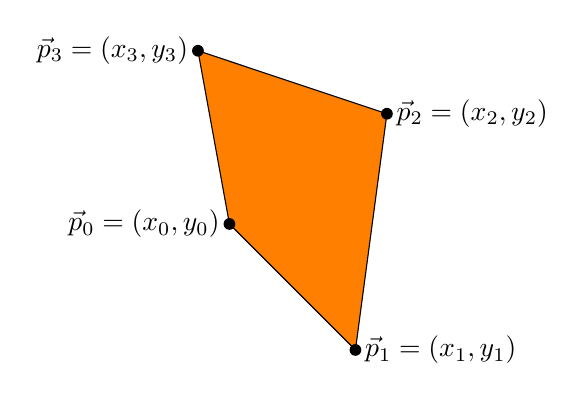
\begin{tikzpicture}[scale=2]
  \coordinate (zero) at (0, 0);
  \coordinate (one) at (0.8, -0.8);
  \coordinate (two) at (1, 0.7);
  \coordinate (three) at (-0.2, 1.1);
  \draw[fill=orange]
    (zero) node[left] {$\vec{p}_0 = (x_0, y_0)$}
    -- (one) node[right] {$\vec{p}_1 = (x_1, y_1)$}
    -- (two) node[right] {$\vec{p}_2 = (x_2, y_2)$}
    -- (three) node[left] {$\vec{p}_3 = (x_3, y_3)$}
    -- cycle;
  \foreach \n in {zero,one,two,three}
    \node at (\n)[circle,fill,inner sep=1.5pt]{};
\end{tikzpicture}

  \textcolor{gray}{\vrule}
  \hspace{0.01\linewidth}
  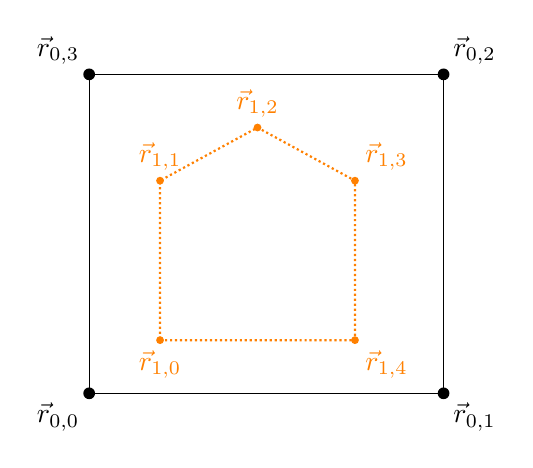
\begin{tikzpicture}[scale=2.25]
  \coordinate (zero) at (0, 0);
  \coordinate (one) at (2.0, 0);
  \coordinate (two) at (2.0, 1.8);
  \coordinate (three) at (0, 1.8);
  \draw
    (zero) node[below left] {$\vec{r}_{0,0}$}
    -- (one) node[below right] {$\vec{r}_{0,1}$}
    -- (two) node[above right] {$\vec{r}_{0,2}$}
    -- (three) node[above left] {$\vec{r}_{0,3}$}
    -- cycle;
  \foreach \n in {zero,one,two,three}
    \node at (\n)[circle,fill,inner sep=1.5pt]{};

  \coordinate (0) at (0.4, 0.3);
  \coordinate (1) at (1.5, 0.3);
  \coordinate (2) at (1.5, 1.2);
  \coordinate (3) at (0.95, 1.5);
  \coordinate (4) at (0.4, 1.2);
  \draw[orange,densely dotted,thick]
    (0) node[below] {$\vec{r}_{1,0}$}
    -- (1) node[below right] {$\vec{r}_{1,4}$}
    -- (2) node[above right] {$\vec{r}_{1,3}$}
    -- (3) node[above] {$\vec{r}_{1,2}$}
    -- (4) node[above] {$\vec{r}_{1,1}$}
    -- cycle;
  \foreach \n in {0,1,2,3,4}
    \node at (\n)[circle,fill,inner sep=1pt,orange]{};
\end{tikzpicture}

  \caption{%
    Simple polygon with four unique vertices is shown on the left hand side.
    A complex polygon with an outer hull
    and an interior hull is shown on the right hand side for comparison.
  }%
  \label{fig:polygon-representation}
\end{figure}

A polygon is considered invalid if one or more of its linear rings are self-intersecting, i.e.\ if any of its rings is considered to be complex.
Data providers frequently provide polygons in invalid states and such polygons must be corrected since they are often not processable by common GIS tools.
Zero-buffering invalid polygons (growing the polygon in all directions by zero units) fixes such problems, as can be seen in~\figref{fig:complex-zero-buffer}.

\begin{figure}[H]
  \centering
  \begin{tikzpicture}[scale=1]
  \coordinate (ll) at (0, 0);
  \coordinate (mid) at (2, 1);
  \coordinate (lr) at (4, 0);
  \coordinate (ur) at (4, 2);
  \coordinate (ul) at (0, 2);
  \draw[fill=orange]
    (ll) node[left] {$\vec{p}_0$}
    -- (ur) node[right] {$\vec{p}_1$}
    -- (lr) node[right] {$\vec{p}_2$}
    -- (ul) node[left] {$\vec{p}_3$}
    -- cycle;
  \foreach \n in {ll,ur,lr,ul}
    \node at (\n)[circle,fill,inner sep=1.5pt]{};

   \draw (4.4, 1) edge[->, thick] node[above] {\texttt{buffer(0.0)}} (6.6, 1);

  \coordinate (offset) at (7, 0);
  \draw[fill=orange]
    ($ (ll) + (offset) $) node[left] {$\vec{p}_0$}
    -- ($ (mid) + (offset) $) node[below] {$\vec{p}_1$}
    -- ($ (lr) + (offset) $) node[right] {$\vec{p}_2$}
    -- ($ (ur) + (offset) $) node[right] {$\vec{p}_3$}
    -- ($ (mid) + (offset) $) node[above] {$\vec{p}_4$}
    -- ($ (ul) + (offset) $) node[left] {$\vec{p}_5$}
    -- cycle;
  \foreach \n in {ll,mid,lr,ur,mid,ul}
    \node at ($ (\n) + (offset) $)[circle,fill,inner sep=1.5pt]{};
\end{tikzpicture}

  \caption{Illustration of how zero-buffering an invalid polygon corrects self-intersecting polygons.}%
  \label{fig:complex-zero-buffer}
\end{figure}

Zero-buffering polygons has the added benefit of normalizing vector data by re-ordering the polygon vertices in an anti-clockwise manner and removing redundant vertices as shown in~\figref{fig:redundant-zero-buffer}.

\begin{figure}[H]
  \centering
  \begin{tikzpicture}[scale=1]
  \coordinate (ll) at (0, 0);
  \coordinate (lm) at (2, 0);
  \coordinate (lr) at (4, 0);
  \coordinate (ur) at (4, 1);
  \coordinate (um) at (2, 1);
  \coordinate (Um) at (2, 2);
  \coordinate (ul) at (0, 1);
  \draw[fill=orange]
    (ll) node[below] {$\vec{r}_0$}
    -- (lm) node[below] {$\vec{r}_1$}
    -- (lr) node[below] {$\vec{r}_2$}
    -- (ur) node[above] {$\vec{r}_3$}
    -- (um) node[above right] {$\vec{r}_4$}
    -- (Um) node[above] {$\vec{r}_5$}
    -- (um) node[above left] {$\vec{r}_6$}
    -- (ul) node[above] {$\vec{r}_7$}
    -- cycle;
  \foreach \n in {ll,lm,lr,ur,um,Um,um,ul}
    \node at (\n)[circle,fill,inner sep=1.5pt]{};

   \draw (4.9, 0.5) edge[->, thick] node[above] {\texttt{buffer(0.0)}} (7.1, 0.5);

  \coordinate (offset) at (8, 0);
  \draw[fill=orange]
    ($ (ll) + (offset) $) node[below] {$\vec{r}_0$}
    -- ($ (lr) + (offset) $) node[below] {$\vec{r}_1$}
    -- ($ (ur) + (offset) $) node[above] {$\vec{r}_2$}
    -- ($ (ul) + (offset) $) node[above] {$\vec{r}_3$}
    -- cycle;
  \foreach \n in {ll,lr,ur,ul}
    \node at ($ (\n) + (offset) $)[circle,fill,inner sep=1.5pt]{};
\end{tikzpicture}

  \caption{Illustration of how zero-buffering polygons removes redundant vertices.}%
  \label{fig:redundant-zero-buffer}.
\end{figure}

This allows you to apply simpler similarity measures for comparing polygons, and reduces computational costs when processing the polygons.
Technical details for applying zero-buffers to vector data is provided in~\appref{app:zero-buffer}.
We will come back to how to combine vector and raster datasets by \textit{rasterization} in~\secref{sec:masking} where it will also become clear why the removal of redundant vertices is of importance.


\topic{Raster data}%
\label{sec:raster-data}
% \usepackage{tikz-3dplot}
% \tdplotsetmaincoords{60}{125}
% \tdplotsetrotatedcoords{0}{0}{0}

\begin{tikzpicture}[scale=3,tdplot_rotated_coords,
                    cube/.style={very thick,black},
                    grid/.style={very thin,gray},
                    axis/.style={->,ultra thick},
                    rotated axis/.style={->,purple,ultra thick}]

    \tikzmath{
      \gridspacing=0.25;
    }
    %draw a grid in the x-y plane
    \foreach \x in {-0.5,0,...,2.5}
        \foreach \y in {-0.5,0,...,2.5}
        {
            \draw[grid,blue,thick] (\x,-0.5,0) -- (\x,2.5,0);
            \draw[grid,blue,thick] (-0.5,\y,0) -- (2.5,\y,0);
        }

    \foreach \x in {-0.5,0,...,2.5}
        \foreach \y in {-0.5,0,...,2.5}
        {
            \draw[grid,green,thick] (\x,-0.5,\gridspacing) -- (\x,2.5,\gridspacing);
            \draw[grid,green,thick] (-0.5,\y,\gridspacing) -- (2.5,\y,\gridspacing);
        }

    \foreach \x in {-0.5,0,...,2.5}
        \foreach \y in {-0.5,0,...,2.5}
        {
            \draw[grid,red,thick] (\x,-0.5,2*\gridspacing) -- (\x,2.5,2*\gridspacing);
            \draw[grid,red,thick] (-0.5,\y,2*\gridspacing) -- (2.5,\y,2*\gridspacing);
        }

    %draw the main coordinate frame axes
    \draw[axis,tdplot_main_coords] (-1.5,-1.5,0) -- (-0.5,-1.5,0) node[anchor=west]{$x$};
    \draw[axis,tdplot_main_coords] (-1.5,-1.5,0) -- (-1.5,-0.5,0) node[anchor=north west]{$y$};
    \draw[axis,tdplot_main_coords] (-1.5,-1.5,0) -- (-1.5,-1.5,1) node[anchor=west]{$z$};

    \node[circle,radius=1,above] at (-0.5, -0.5, 2*\gridspacing) {$test$};
\end{tikzpicture}


\subsection{Data sets}%
\label{sec:data-sets}

The modelling results presented in~\secref{sec:experiments} are trained on GIS data covering the Norwegian municipality of Trondheim.
All data sets have been made available by the \enquote{Norge digitalt}-partnership and have been downloaded from \url{https://geonorge.no}, an online service hosted by \textit{Norwegian Mapping and Cadastre Authority} (\textit{Statens Kartverk}).
All data, unless otherwise stated, are licenced under the \enquote{Norge digitalt}-licence\footnote{Information regarding the \enquote{Norge digitalt}-licence can be found here:\\ \url{https://www.geonorge.no/Geodataarbeid/Norge-digitalt/Avtaler-og-maler/Norge-digitalt-lisens/}.} which restricts the use to non-commercial purposes.

\topic{Raster data sets}
\begin{figure}[htb]
  \includegraphics[width=0.75\linewidth]{data/rgb-example}
\end{figure}

\begin{figure}[htb]
  \includegraphics[width=0.75\linewidth]{data/lidar-example}
\end{figure}

\begin{table}[htb]
  \centering
  \resizebox{\textwidth}{!}{%
    \begin{tabular}{lSSrrrr}
      \toprule
      {Data set} & {Resolution} & {Size} & {Coverage area} & {Date} & Scan angle & Accuracy \\
      \midrule
      Orthophoto~\cite{trondheim_ortophoto_2017} & \SIrange{0.04}{0.15}{\meter} & \SI{161}{\giga\byte}  & TODO & \date{2017} & {} & \SI{\pm 0.35}{\meter} \\
      LiDAR~\cite{trondheim_lidar_2017} & \SI{0.2}{\meter} & \SI{25}{\giga\byte} & \SI{342}{\kilo\meter\squared} & \date{2017-10-10} & \SI{\pm 20}{\degree} & \SI{\pm 0.02}{\meter} (SD) \\
      \bottomrule
    \end{tabular}%
  }
\end{table}

\begin{table}[htb]
  \centering
  \begin{tabular}{cc}
    \toprule
    {Point density (\si{\per\meter\squared})} & {Proportion (\%)} \\
    \midrule
    $> 100\%$ & 97.7 \\
    \SIrange{85}{100}{\percent} & 1.2 \\
    \SIrange{60}{85}{\percent} & 1.1 \\
    \bottomrule
  \end{tabular}
  \caption{
    Control of point cloud density of the Trondheim 2017 LiDAR data set.
    The densities are calculated within rolling windows of size $\SI{10}{\meter} \times \SI{10}{\meter}$~\cite{trondheim_lidar_2017}.
    }
\end{table}

Pixel domain is $(1, 254)$ for all three color channels.
\SI{70.77}{\percent} of all pixels are valid, probably due to lower resolution than the actual resolution.
Elevation data is in domain $(-9.390, 569.050)$.


\topic{Vector data sets}
The \enquote{Matrikkelen - Eiendomskart Teig}\footnote{Product specification for \enquote{Matrikkelen - Eiendomskart Teig} can be found here:\\\url{https://kartkatalog.geonorge.no/metadata/74340c24-1c8a-4454-b813-bfe498e80f16}.} data set contains all cadastral plots in Trondheim, the use of which will be explained in~\secref{sec:tiling-algorithm}.
The \enquote{FKB-bygning}\footnote{Product specification for \enquote{FKB-bygning} can be found here:\\\url{https://kartkatalog.geonorge.no/metadata/8b4304ea-4fb0-479c-a24d-fa225e2c6e97}.} data set contains all registered building outlines in Trondheim.
The building outlines will be used to construct binary classification masks as outlined in~\secref{sec:masking-algorithm}.
Both data sets are illustrated in~\figref{fig:vector-data-example}.

\begin{figure}[htb]
  \includegraphics[trim={5cm 0 5cm 0},clip, width=0.49\linewidth]{data/teig-example}
  \includegraphics[trim={5cm 0 5cm 0},clip, width=0.49\linewidth]{data/building-example}
  \caption{%
    Illustration of vector data sets.
    Cadastral plots are shown on the left while building outlines are shown on the right.
    \copyright{Kartverket}.
  }%
  \label{fig:vector-data-example}
\end{figure}


\subsection{Tiling Algorithm}%
\label{sec:tiling-algorithm}
Given a specific geographic region, defined by the extent of the cadastral plot, we must retrieve the raster which entirely covers the region of interest.
The simplest approach is to calculate the \textit{axis-aligned bounding box} of the plot, the minimum-area enclosing rectangle of the given plot, defined by four points, $(x_{\mathrm{min}}, y_{\mathrm{min}}, x_{\mathrm{max}}, y_{\mathrm{max}})$.
The resulting bounding box of width $w = x_{\mathrm{max}} - x_{\mathrm{min}}$ and height $h = y_{\mathrm{max}} - y_{\mathrm{min}}$ is shown in \figref{fig:cadastral-bbox}.

\begin{figure}[htb]
  \captionsetup[subfigure]{position=b}
  \centering
  \subcaptionbox{
    Bounding box calculation for a given cadastral.
    The cadastral is drawn in \textcolor{orange}{orange},
    and the resulting bounding box is drawn with \textcolor{blue}{blue} dashed lines.
    \label{fig:cadastral-bbox}
  }{
    \begin{tikzpicture}[scale=0.07]
  \tikzmath{
    \xmin=0;
    \xmax=100;
    \ymin=0;
    \ymax=100;
    \xmid=0.5 * \xmin + 0.5 * \xmax;
    \ymid=0.5 * \ymin + 0.5 * \ymax;
  }
  \coordinate (lr) at (\xmax, \ymin);
  \coordinate (ul) at (\xmin, \ymax);

  \filldraw[cadastralcolor!40, draw=black] (50, \ymin) -- (62.5, 12.5) -- (25, 50) -- (\xmax, 50) -- (50, \ymax) -- (0, 50) -- cycle;
  \draw[dashed, color=cadastralcolor] (\xmin, \ymin) rectangle (\xmax, \ymax);

  \draw (ul) node[below right] {$(x_{\mathrm{min}}, y_{\mathrm{max}})$};
  \fill[cadastralcolor] (ul) circle [radius=1];

  \draw (lr) node[above left] {$(x_{\mathrm{max}}, y_{\mathrm{min}})$};
  \fill[cadastralcolor] (lr) circle [radius=1];

  \draw (\xmid, \ymax) node[above] {$w = x_{\mathrm{max}} - x_{\mathrm{min}}$};
  \draw (\xmax, \ymid) node[above, rotate=-90] {$h = y_{\mathrm{max}} - y_{\mathrm{min}}$};

  \draw (\xmid, 65) node[scale=1.5, black] {\textsf{CADASTRAL}};
\end{tikzpicture}

  }
  \hspace{2em}
  \subcaptionbox{
    Figure showing the difference between a regular bounding box shown in
    \textcolor{blue}{blue}, and a minimum rotated rectangle shown in
    \textcolor{red}{red}.
    Angle of rectangle rotation denoted by $\phi$.
    \label{fig:rotated-bbox}
  }{
    \begin{tikzpicture}[scale=0.04]
  \tikzmath{
    \xmin=0;
    \xmax=100;
    \ymin=0;
    \ymax=100;
    \xmid=0.5 * \xmin + 0.5 * \xmax;
    \ymid=0.5 * \ymin + 0.5 * \ymax;
  }
  \coordinate (lr) at (\xmax, \ymin);
  \coordinate (ul) at (\xmin, \ymax);

  \draw[dashed, color=cadastralcolor, fill=cadastralcolor!20] (\xmin, \ymin) rectangle (\xmax, \ymax);
  \draw[dashed, color=red, fill=red!20, fill opacity=1] (\xmin, 50) -- (50, \ymin) -- (\xmax, 50) -- (50, \ymax) -- cycle; 
  \filldraw[orange, draw=black] (50, \ymin) -- (62.5, 12.5) -- (25, 50) -- (\xmax, 50) -- (50, \ymax) -- (0, 50) -- cycle;
  \draw[dashed, thick, color=red] (\xmin, 50) -- (50, \ymin) -- (\xmax, 50) -- (50, \ymax) -- cycle; 

  \fill[cadastralcolor] (ul) circle [radius=1];
  \fill[cadastralcolor] (lr) circle [radius=1];

  \fill[red] (\xmin, 50) circle [radius=1];
  \fill[red] (\xmax, 50) circle [radius=1];

  % Draw angle of rotation
  \draw[black] (\xmid + 20, \ymax) arc [start angle=0, end angle=-45, radius=20] node[midway, right] {$\phi$};

  % The following is added such that the resulting figure has the same dimensions as cadastre_bbox
  \draw (ul) node[above] {$(x_{\mathrm{min}}, y_{\mathrm{max}})$};
  \fill[cadastralcolor] (ul) circle [radius=1];
  \draw (lr) node[below] {$(x_{\mathrm{max}}, y_{\mathrm{min}})$};
  \fill[cadastralcolor] (lr) circle [radius=1];
\end{tikzpicture}

  }
\end{figure}

The edges of the bounding box is by definition oriented parallel to the coordinate axes.
An alternative method is to calculate the \textit{arbitrarily oriented minimum bounding box} (AOMBB), a rectangle rotated by $\phi$ degrees w.r.t. the $x$-axis, as shown in \figref{fig:rotated-bbox}.

While AOMBB results in a region with less superfluous raster data, it requires warping of the original raw raster when $\phi \not\in \{ \SI{0}{\degree}, \SI{90}{\degree}, \SI{180}{\degree}, \SI{270}{\degree} \}$.
This requires data interpolation of the original raster data due to the rotation of the coordinate system, and may introduce artifacts in the warped raster data without careful parameter tuning.
AOMBB is therefore not a viable approach during the preprocessing stage, and we will therefore use axis-aligned minimum bounding boxes instead, from now on simply referred to as \textit{bounding boxes}.

Calculating bounding boxes for the cadastral plots in our data sets will yield rectangles of variable dimensions.

\begin{figure}[htb]
  \includegraphics[width=\linewidth]{bbox_stats}
\end{figure}

\begin{align*}
  \vec{r^*} &= (w^*, h^*),
  \\
  \text{ where }
  h^* &:= \ceil{\frac{h}{\SI{64}{\meter}}} \cdot \SI{64}{\meter},
  w^* := \ceil{\frac{w}{\SI{64}{\meter}}} \cdot \SI{64}{\meter}
\end{align*}

\begin{figure}[H]
  \centering
  \begin{tikzpicture}[scale=0.035]
  \tikzmath{
    \tile=64;
    \bboxwidth=2.25 * \tile;
    \collectionwidth=3 * \tile;
    \bboxheight=1.25 * \tile;
    \collectionheight=2 * \tile;
    \offset = 0.375 * \tile;
    \shift = 5;
  }
  \draw (0, 0) grid[step=\tile] (\collectionwidth, \collectionheight);

  % Show tile dimensions
  \draw[decoration={brace}, decorate]
    (-\shift, 0) -- node[above left] {$\SI{64}{\metre}~$} node[below left] {$\SI{256}{\pixel}$} (-\shift, \tile);

  \draw[decoration={brace,mirror}, decorate]
    (0, -\shift) -- node[below=2pt, align=center] {$\SI{64}{\metre}$ \\ $\SI{256}{\pixel}$} (\tile, -\shift);

  % Show dimensions of tile collection
  \draw[decoration={brace,mirror}, decorate]
    (\collectionwidth + \shift, 0) 
    --
    node[right=2pt]{$h^*$}
    (\collectionwidth + \shift, \collectionheight);
  \draw[decoration={brace}, decorate]
    (0, \collectionheight + \shift) 
    --
    node[above=2pt]{$w^*$}
    (\collectionwidth, \collectionheight + \shift);

  % Arrows showing growth of bounding box
  \tikzset{>=latex}
  \draw (\bboxwidth + \offset + 1, \offset - 1) edge[->, thick, dashed] (\collectionwidth - 1, 1);
  \draw (\bboxwidth + \offset + 1, \bboxheight + \offset + 1) edge[->, thick, dashed] (\collectionwidth - 1, \collectionheight - 1);
  \draw (\offset - 1, \bboxheight + \offset + 1) edge[->, thick, dashed] (1, \collectionheight);
  \draw (\offset - 1, \offset - 1) edge[->, thick, dashed] (1, 1);

  % Draw original bounding box
  \draw[dotted, thick, color=cadastralcolor, fill=cadastralcolor!10, fill opacity = 0.9] (0 + \offset, 0 + \offset) rectangle (\bboxwidth + \offset, \bboxheight + \offset);
\end{tikzpicture}

\end{figure}


\subsection{Masking Algorithm}%
\label{sec:masking-algorithm}
\begin{figure}[H]
  \centering
  \begin{tikzpicture}[every node/.style={minimum size=0.6*1.3cm-\pgflinewidth, outer sep=0pt, fill=orange!80, fill opacity=0.4}, scale=0.6*1.3]
  \tikzmath{
    \gridheight=4;
    \gridwidth=4;
  }

  \def\cells{
    (0.5,0.5),
    (1.5,1.5),
    (2.5,2.5),
    (3.5,3.5),
    (3.5,2.5),
    (3.5,1.5),
    (3.5,0.5),
    (2.5,0.5),
    (1.5,0.5),
    (2.5,1.5),
    (2.5,3.5),
    (1.5,2.5)
  };
  \coordinate (offset) at (0.5, 0.5);
  \foreach \cell in \cells {
    \node at ($(\cell$) {};
  }

  \draw[step=1,color=black,draw opacity=0.6] (0,0) grid (\gridwidth,\gridheight);
  \draw[thick, orange, line width=0.1cm] (0.5, 0)
    -- (3.33, \gridheight)
    -- (\gridwidth, \gridheight)
    -- (\gridwidth, 0)
    -- cycle;
\end{tikzpicture}

  \hspace{2em}
  \input{tikz/non_touching_mask.tex}
  \caption{
    The same polygon discretized to a raster grid using two different techniques.
    In the left figure, all pixels being \textit{touched} by the interior of the polygon
    are considered a part of the polygon, while in the left figure, only pixels
    entirely \textit{contained} within the interior are considered being part
    of the polygon.
  }
\end{figure}


\subsection{Raster Normalization}%
\label{sec:raster-normalization}
Input data normalization has been found to be of vital importance when training neural networks, in certain cases reducing predictive errors by several orders of magnitude and training times by one order of magnitude \cite{input_normalization_1997}.
How to normalize input data depends on distribution of the feature space, which will be investigated here.

\todo{Find paper investigating the effect of data normalization on CNNs.}

\subsubsection*{RGB rasters}

A given RGB pixel is an unsigned 8-bit integer and therefore takes values in a bounded, integer domain
%
\begin{equation*}
  I_{i,j,c} \in \{0, 1, ..., 255\}, \text{ for } c \in \{r, g, b\}.
\end{equation*}
%
The distribution of each color channel over the entire coverage area of the Trondheim aerial photography data set is shown in \figref{fig:rgb-density}, and aggregate statistics for each channel are listed in \tabref{tab:rgb-statistics}.

\begin{figure}[htb]
  \begin{floatrow}
    \ffigbox[9cm]{%
      \includegraphics[width=\linewidth]{rgb-density}
    }{%
      \caption{
        Distribution density for all three color channels in the aerial photography data set covering Trondheim municipality (2017).
        %Peak at 64 and 191.
      }
      \label{fig:rgb-density}
    }
    \inlinetable{%
      \scalebox{0.75}{
        \begin{tabular}{
          l
          S[round-mode=places, round-precision=2]
          S[round-mode=places, round-precision=2]
        }
          \toprule
          {Image channel} & {Mean [1]} & {SD [1]} \\
          \midrule
          \textcolor{red}{Red} & 101.60925940814 & 55.010463592563 \\
          \textcolor{green}{Green} & 102.67104002891 & 48.740409963323 \\
          \textcolor{blue}{Blue} & 91.286001382234 & 37.216349915699 \\
          \bottomrule
        \end{tabular}
      }
      \vspace{5em}
    }{%
      \caption{
        Aggregate statistics for each image channel distribution for the aerial photography data set covering Trondheim municipality (2017).
      }
      \label{tab:rgb-statistics}
    }
  \end{floatrow}
\end{figure}

The RGB pixels can be normalized to the $[0, 1]$ domain by dividing by $255$ across all three image channels.
This is in essence a lossless transformation, since the normalization function $f(x) = x/255$ is trivially invertible, and thus no information is lost by this normalization.

\subsubsection*{LiDAR rasters}

The $z$ channel in our image input represents elevation data from the digital surface model.
Elevation pixels are represented by 32-bit, single-precision floating point numbers, and can theoretically take values in the domain
%
\begin{equation*}
  I_{i,j,z} \in (-3.4 \times 10^{38}, 3.4 \times 10^{38}).
\end{equation*}

\begin{figure}[htb]
  \begin{floatrow}
    \ffigbox[9cm]{%
      \includegraphics[width=\linewidth]{elevation-density}
    }{%
      \caption{
        Distribution density for elevation data set covering Trondheim municipality (2017).
        Outlier values $(\SI{0}{\meter}, \SI{2.74}{\percent})$ and $(\SI{148}{\meter}, \SI{1.93}{\percent})$ have been excluded.
      }
      \label{fig:elevation-density}
    }
    \inlinetable{%
      \scalebox{0.75}{
        \begin{tabular}{
          l
          S[round-mode=places, round-precision=2]
          S[round-mode=places, round-precision=2]
        }
          \toprule
          {Image channel} & {Mean [m]} & {SD [m]} \\
          \midrule
          Elevation & 155.36339532445 & 116.52777315076 \\
          \bottomrule
        \end{tabular}
      }
      \vspace{7em}
    }{%
      \caption{
        Aggregate statistics for elevation data set covering municipality of Trondheim (2017).
      }
      \label{tab:elevation-statistics}
    }
  \end{floatrow}
\end{figure}

It is infeasible to normalize this domain to $[0, 1]$ like the RGB normalization, it would yield large floating point errors and vanishingly small values.

The digital surface model providing elevation data in form of the $z$ channel in our raster inputs is \textit{not} bounded by any domain, at least not theoretically.
~
\begin{align*}
  &\text{Theoretically:} ~ I_{i,j,z} \in (-\infty, \infty)
  \\
  &\text{Numerically:} ~ I_{i,j,z} \in (-3.4 \times 10^{38}, 3.4 \times 10^{38})
  \\
  &\text{Practically:} ~ I_{i,j,z} \in (-432.65, 8848)
\end{align*}

